\chapter{Semantic Mapping}\label{chap:semantic-mapping}

% Reasoning on why to use semantic mapping
% High-level processing
Also due to uncertainity and complexity 
% Advantages of Multi-modal approaches
% 

It is therefore not only for efficiency reasons but also desirable to handle
the information on an high-level probabilistic fashion.



\section{Dora Architecture Overview}
This thesis motivation lies on developing methods for detecting knowledge gaps
on the semantic knowledge of a mobile agent. For that the semantic mapping system
proposed by \cite{pronobis2011phd} was used as a base.

Pronobis presents a system architecture working on indoor environments using
non\hyp{}omnidirectional lasers and visual sensors, that by integrating cues such as geometry,
object presence and appearances is able to perform inference across any semantic property,
for example to handle place categorization.
The introduced semantic representation has not only been tested on real scenarios
and performance measured across several conditions~\cite{pronobis2007iros} but also shown
to be tailored to effectively solve tasks arising on mobile robotics~\cite{hanheide2011ijcai}.
Besides that the system architecture has been drawn with an high-focus on probabilistic
and uncertain reasoning, human interaction and life-long learning capabilities.

For that it was considered an excellent base defining not only the concepts and
requirements of an high-level semantic representation but also the information flow
between all the layers involved on the agent.
The system is implemented on \Gls{Dora} and a brief overview of its architecture is
given in the following sections.

\subsection{System organization}
The \Gls{Dora} system~\cite{hanheide2011ijcai} consists of several co-operating
sub-systems, all of which actively use or maintain the spatial knowledge representation
(see \autoref{fig:dora-architecture}):

\begin{figure}[h]
\centering
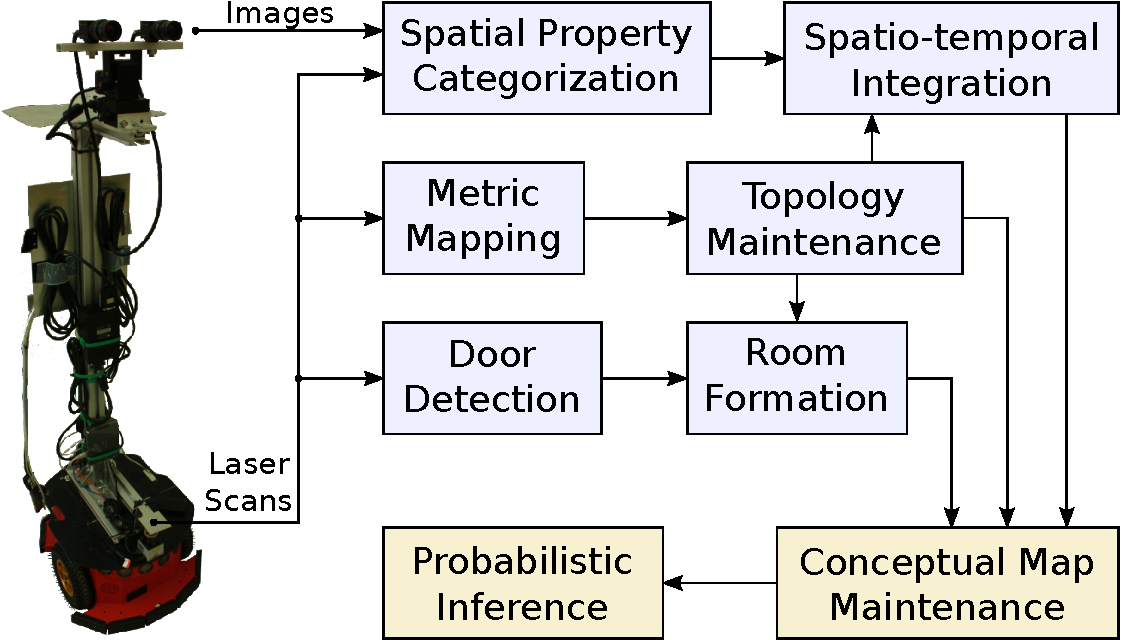
\includegraphics[width=0.7\textwidth]{figures/dora-architecture.pdf}
\caption{\label{fig:dora-architecture}Interaction of the sub-systems
         in Dora with special focus on the conceptual layer.}
\end{figure}

\subsubsection*{Sensory Layer}
The sensory layer is responsible for all the low-level sensors.
It maintains an immediate and exact description of the environment by using
data such as images from cameras, 2D\hyp{}laser scans and odometry from encoders in the
movement motors. The information provided by it is used on the higher layers to extract
tractable information.

\subsubsection*{Place Layer}
The place layer is responsible for discretizing the continuous low-level space into
a finite number of places by spreading several virtual places markers around the whole
environment and maintaining connectivity information between them.
This virtual places also handle information associating the robot view point. Together
with extracted properties they allow the system to perform a clever integration over the
room properties, avoiding sampling bias, for example coming due to the robot spend too
much time in a part of the room~\cite{pronobis2010ijrr}.

\subsubsection*{Categorical Layer}
The categorical layer is responsible for extracting high-level information from the
sensors. It has classifiers trained to detect several properties from the visual and laser
features captured on the sensory layer.
It is responsible for detecting objects, doors, categorize the geometry and the appearance.
The used methods and properties extracted by this layer are described in more detail in
\autoref{sec:dora-features}.

\subsubsection*{Conceptual Layer}
The conceptual layer merges the sensed properties and places structure together
with general knowledge under a unified probabilistic semantic representation: the
\emph{conceptual map}.
This conceptual map is the structure for handling the high-level semantic information
and performing inferences. It is the layer where the novelty detection methods described
on this thesis are meant to be integrated and is described in more detail in
\autoref{sec:conceptual-map}.


\subsection{Features}
\label{sec:dora-features}


\section{Conceptual Map}
\label{sec:conceptual-map}
As \gls{Dora} moves through the environment its \emph{conceptual layer} builds a structural and
probabilistic representation of the space instantiated as a \emph{graphical model}.
It includes taxonomy of human\hyp{}compatible spatial concepts which are linked to the sensed 
instances of these concepts drawn from lower layers. It is the conceptual layer which 
contains the information that kitchens commonly contain cereal boxes and have certain 
general appearance and allows the robot to infer that the cornflakes box in front of the 
robot makes it more likely that the current room is a kitchen. The conceptual layer is 
described in terms of a probabilistic ontology defining spatial concepts and linking 
those concepts to instances of spatial entities (see the example of the ontology in
\autoref{fig:dora-architecture}).

Based on this design, a \emph{chain graph} model is proposed as a 
representation for performing inferences on the knowledge represented in the conceptual 
layer. Chain graphs are probabilistic graphical models that combine the properties of 
both Bayesian Networks and Random Markov Fields. This results in an efficient approach to 
probabilistic modeling and reasoning about conceptual knowledge.

\begin{figure}[h]
\centering
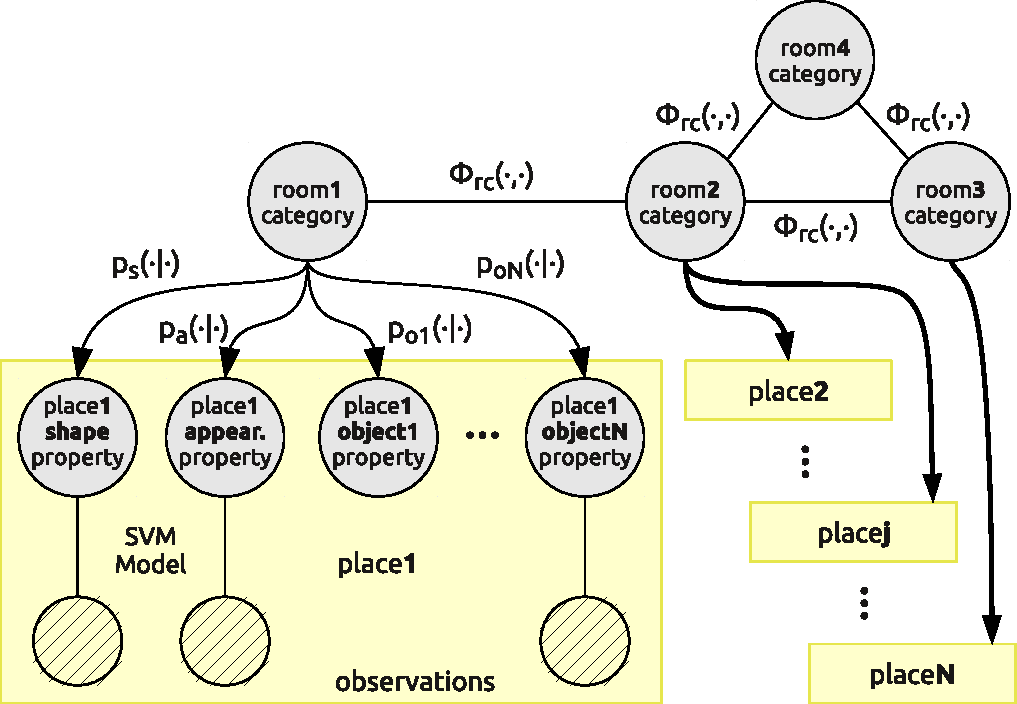
\includegraphics[width=0.75\textwidth]{figures/chaingraph.pdf}
\caption{\label{fig:chain-graph}Example chain-graph produced by the \emph{conceptual layer}.}
\end{figure}

%The conceptual layer structures the sensed environment together with the conceptual knowledge
%in order to create a structured probabilistic representation of the world.
An exemplary chain graph corresponding to the conceptual map ontology is presented
in \autoref{fig:chain-graph}. 
Each discrete place identified in the environment is represented by a set of random variables, 
one for each class of relation linked to that place. These are each connected to a random variable
over the categories of rooms, representing the ``is-a'' relation between rooms and their categories. 
Moreover, the room category variables are connected by undirected links to one another according 
to the topological map. The remaining variables represent: shape and appearance properties of space 
as observed from each place, and the presence of objects. 
These are connected to observations of features extracted directly from 
the sensory input. Finally, the 
distributions $p_{s}(\cdot|\cdot)$, $p_a(\cdot|\cdot)$, $p_{o_i}(\cdot|\cdot)$ 
represent the common sense knowledge about shape, appearance, and object co-occurrence, respectively. 
They allow for inference about other properties and room categories e.g. that the room is likely to be a kitchen,
because you are likely to have observed cornflakes in it. 

The use of graphical models to describe distributions of variables has useful properties.
First, they permit inference about uncertain conceptual knowledge. At the same time, they are 
generative models and therefore allow to calculate the probability
on any given subset of variables of the graph, allowing the system to work even when some
information is missing.

\subsection{Factor Graphs}
Although the conceptual layer works with \emph{chain graphs}~\cite{lauritzen2002chain},
those can be converted into \emph{factor graphs}~\cite{kschischang2001factor}.
Factor graphs have been introduced in \autoref{sec:graphical-models} and are used
throughout this thesis as they provide a easier manipulation due to factorization.

Moreover, there exists efficient implementation of inference engines operating on factor
graph representations~\cite{Mooij_libDAI_10}.
Describing the distribution function in terms of graphs allows to use those engines to
efficently calculate marginals on any given subset of variables by exploiting conditional
independence between variables.

\subsection{Uncertain Sensing and Implicit Factors}
\label{sec:cues-from-low-level}
In a realistic scenario classification tasks are by their nature uncertain.
And although a trained classifier is able to decide which class is more likely, there is
interest in handling uncertainty produced by those to turn decisions more robust.

By modelling the classifiers as an implicit function $\phi_{classifier}(c, x)$ it becomes
possible to model the uncertainty of those given the presence of the sensed low-level
features $X$. The presence of those implicit models no longer allow to calculate the
normalization factor over the whole graph as there is no explicit model for either the
low\hyp{}level features $X$ (e.g.\ $X$ can be an image received from a visual sensor)
or for $\phi_{classifier}$ (e.g.\ the classifier can be an \gls{SVM}).

Nonetheless it is still possible to calculate any probability given that the features $X$
are observed. For that instead of modelling the variables $X$ and explicitly describing
the factor $\phi_{classifier}$ it is enough to replace it by an observed factor $\phi_{classifier}(c|x)$.


\begin{figure}[h]
\centering
\subfloat[]{
\begin{tikzpicture}
  \node [matrix,matrix anchor=mid, column sep=20pt, row sep=10pt,ampersand replacement=\&] {
    \& \& \node (graph) [] {\dots}; \& \& \\
    \& \& \node (prop) [latent] {$c$}; \& \& \\
    \& \& \node (fac) [factor] {}; \& \& \\
    \& \& \& \& \\
    \node (x1) [obs] {$x_1$}; \&
    \node (x2) [obs] {$x_2$}; \&
    \node (x3) [obs] {$x_3$}; \&
    \node (xi) [] {\dots}; \&
    \node (xn) [obs] {$x_n$}; \\
  };
  \draw [-] (prop) -- (graph);
  \draw [-] (prop) -- (fac);
  \draw [-] (fac) -- (x1);
  \draw [-] (fac) -- (x2);
  \draw [-] (fac) -- (x3);
  \draw [-] (fac) -- (xi);
  \draw [-] (fac) -- (xn);

  \node (captfactor) [right=2pt of fac] {\footnotesize{$\phi_{classifier}(c, x)$}};
\end{tikzpicture}
}
\qquad
\subfloat[]{
\begin{tikzpicture}
  \node [matrix,matrix anchor=mid, column sep=20pt, row sep=10pt,ampersand replacement=\&] {
    \& \& \node (graph) [] {\dots}; \& \& \\
    \& \& \node (prop) [latent] {$c$}; \& \& \\
    \& \& \node (fac) [factor] {}; \& \& \\
    \& \& \node (hidden) [latent,draw=none] {}; \& \& \\
  };
  \draw [-] (prop) -- (graph);
  \draw [-] (prop) -- (fac);
  \node (captfactor) [right=2pt of fac] {\footnotesize{$\phi_{classifier}(c | x)$}};
\end{tikzpicture}

}

\caption{\label{fig:implicit-factor}By modelling classifiers as implicit factors it is
possible to perform inference on the graphical models handling the uncertainty measures
produced by those classifiers.}
\end{figure}

